\documentclass[10pt, conference, compsocconf]{IEEEtran}
\usepackage{xcolor}
\usepackage{mathtools}
\usepackage{enumerate}
\usepackage{hyperref}
\usepackage{amssymb}
\usepackage{subfig}
\usepackage{amsmath}
\usepackage{eqnarray}
\usepackage[]{algorithm}
\usepackage{clrscode3e}
\usepackage[pdftex]{graphicx}

\DeclarePairedDelimiter{\ceil}{\lceil}{\rceil}

\begin{document}

%%%%%%%%%%%%%%%%%%%%%%%%%%%%%%%%%%%%%%%%%%%%%%%%%%%%%%%%%%%%%%%%%%%%%%%
%%%%%%%%%%%%%%%%%%%%%%%%%%%%%%%%%%%%%%%%%%%%%%%%%%%%%%%%%%%%%%%%%%%%%%%
%%
%% TITLE
%%
%%%%%%%%%%%%%%%%%%%%%%%%%%%%%%%%%%%%%%%%%%%%%%%%%%%%%%%%%%%%%%%%%%%%%%%
%%%%%%%%%%%%%%%%%%%%%%%%%%%%%%%%%%%%%%%%%%%%%%%%%%%%%%%%%%%%%%%%%%%%%%%

\title{A Parallel Watershed Algorithm for $N$--dimensional Affinity
  Graphs by Merging Local Watersheds}

\author{
Aleksandar Zlateski\\ Massachusetts Institute of Technology\\ Cambridge, MA\\
{\tt\small zlateski@mit.edu}
\and
H. Sebastian Seung\\ Princeton University\\ Princeton, NJ\\
{\tt\small sseung@princeton.edu}
}



\maketitle
%\thispagestyle{empty}

%%%%%%%%%%%%%%%%%%%%%%%%%%%%%%%%%%%%%%%%%%%%%%%%%%%%%%%%%%%%%%%%%%%%%%%
%%%%%%%%%%%%%%%%%%%%%%%%%%%%%%%%%%%%%%%%%%%%%%%%%%%%%%%%%%%%%%%%%%%%%%%
%%
%% ABSTRACT
%%
%%%%%%%%%%%%%%%%%%%%%%%%%%%%%%%%%%%%%%%%%%%%%%%%%%%%%%%%%%%%%%%%%%%%%%%
%%%%%%%%%%%%%%%%%%%%%%%%%%%%%%%%%%%%%%%%%%%%%%%%%%%%%%%%%%%%%%%%%%%%%%%


\begin{abstract}
Abstract
\end{abstract}

%%%%%%%%%%%%%%%%%%%%%%%%%%%%%%%%%%%%%%%%%%%%%%%%%%%%%%%%%%%%%%%%%%%%%%%
%%%%%%%%%%%%%%%%%%%%%%%%%%%%%%%%%%%%%%%%%%%%%%%%%%%%%%%%%%%%%%%%%%%%%%%
%%
%% INTRODUCTION
%%
%%%%%%%%%%%%%%%%%%%%%%%%%%%%%%%%%%%%%%%%%%%%%%%%%%%%%%%%%%%%%%%%%%%%%%%
%%%%%%%%%%%%%%%%%%%%%%%%%%%%%%%%%%%%%%%%%%%%%%%%%%%%%%%%%%%%%%%%%%%%%%%

\section{Introduction}


\section{Watershed Transform Algorithm}

Inspired by the \emph{drop of water principle}~\cite{Cousty2009} we
define a steepest descent discrete dynamics on a connected
edge-weighted graph $G=(V,E)$ with non-negative weights. A water drop
travels from a vertex to another vertex using only \emph{locally
  minimal} edges. An edge $\{u,v\}$ is \emph{locally minimal} with
respect to $u$ if there is no edge in $E$ incident to $u$ with lower
weight. Starting from a vertex $v_{0}$ the evolution of the system can
be represented as a \emph{steepest descent walk} $\left\langle
v_{0},e_{0},v_{1},e_{1},v_{2}, \dots \right\rangle$ where every edge
$e_{i}$ is locally minimal with respect to $v_{i}.$ A \emph{regional
  minimum $M$} is a connected subgraph of $G$ such that there is a
\emph{steepest descent walk} between any pair of vertices in $M$, and
every \emph{steepest descent walk} in $G$ starting from a vertex in
$M$ will stay within $M$. A vertex $v$ belongs to the \emph{basin of
  attraction} of a \emph{regional minimum $M$} if there exists a
\emph{steepest descent walk} from $v$ to any vertex in $M$. Note that
$v$ can belong to \emph{basins of attractions} of multiple
\emph{regional minima}. In our \emph{watershed transform} we partition
$V$ into \emph{basins of attraction} of \emph{the regional
  minima}. Vertices belonging to more than one \emph{basin of
  attraction} will be referred to as \emph{border vertices} and will
be assigned to one of the \emph{basins} as described below.

\begin{figure}
  \centering
  \subfloat[]{\protect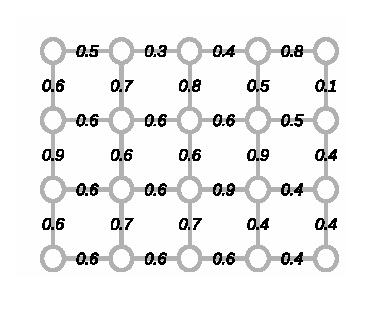
\includegraphics[scale=0.66]{fig/affinity_graph}}
  \subfloat[]{\protect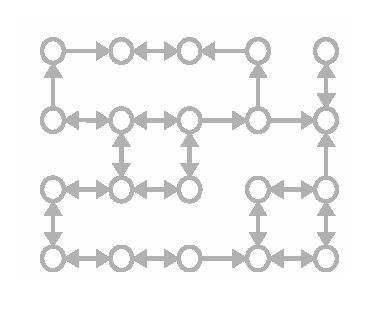
\includegraphics[scale=0.66]{fig/sd_graph}}\\
  \subfloat[]{\protect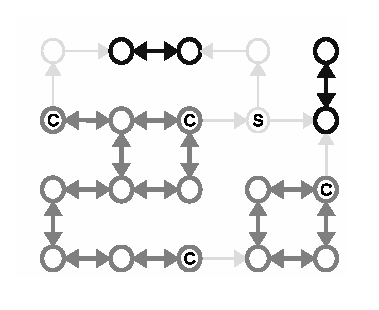
\includegraphics[scale=0.66]{fig/sd_graph_plateaus}}
  \subfloat[]{\protect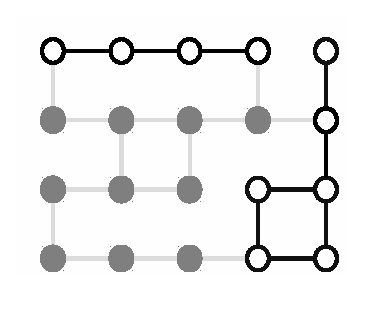
\includegraphics[scale=0.66]{fig/ws_result}}

  \protect\caption{(a) A disaffinity graph; (b) derived steepest
    descent graph; (c) locally minimal plateaus (black), non-minimal
    plateau (dark gray), saddle vertex (S), plateau corners (C); (d)
    the two basins of attractions and border vertices (dark gray)}
\end{figure}


\subsection{Steepest descent graph}

The central quantity in the watershed algorithm is the steepest
descent graph, defined as follows. Consider an undirected weighted
graph $G$ (Fig. 1(a)). Define the directed graph $G'$ in which each
undirected edge of $G$ is replaced by both directed edges between the
same vertices. The \emph{steepest descent graph} $D$ (Fig. 1(b)) is a
subgraph of $G'$ with the property that $D$ includes every edge of
$G'$ with minimal weight of all edges outgoing from the same vertex. A
directed path in $D$ is a path of steepest descent in $G$. The
steepest ascent graph can be defined analogously using edges of
maximal weight. Either steepest ascent or descent can be used without
loss of generality. For simplicity, for a given vertex $v$ we will
refer to its edges in $D$ as incoming, outgoing, and bidirectional. A
\emph{plateau} is a connected component of the subgraph of $D$
containing only bidirectional edges. A \emph{plateau corner} is a
vertex of a \emph{plateau} that has at least one outgoing
edge. \emph{Locally minimal plateaus} contain no \emph{plateau
  corners,} they are equivalent to the regional minima of the original
graph. \emph{Non-minimal plateaus} contain one or more \emph{plateau
  corners}. A \emph{saddle vertex} has more than one outgoing edge. In
Fig. 1(c) we show \emph{locally minimal plateaus }(black),
\emph{non-minimal plateau} (dark gray), \emph{plateau corners} (C),
and a\emph{ saddle vertex} (S).

\subsection{Assigning border vertices}

In Fig. 1(d) we show the \emph{basins of attraction} of the two
\emph{regional minima}. The \emph{border} vertices are shown in dark
gray and belong to both \emph{basins of attraction}. Watershed
cuts~\cite{Cousty2009,Cousty2010} assign \emph{border} vertices with a
single constraint that all the \emph{basins of attraction} have to be
connected. We introduce additional constrains. The watershed transform
has to be uniquely defined and the \emph{non-minimal plateaus} should
be divided evenly. More specifically, we want our dynamics to be
uniquely defined at \emph{saddle vertices, and }the vertices of the
\emph{non-minimal plateaus} to be assigned to the same \emph{basin of
  attraction} as the nearest \emph{plateau corner - }a \emph{plateau
  corner} reachable in fewest steps following the rules of our
dynamics.

\begin{figure}
  \centering
  \subfloat[]{\protect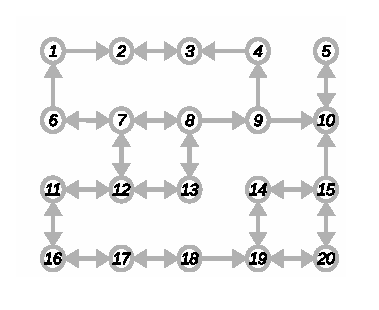
\includegraphics[scale=0.66]{fig/sd_graph_ordered}}
  \subfloat[]{\protect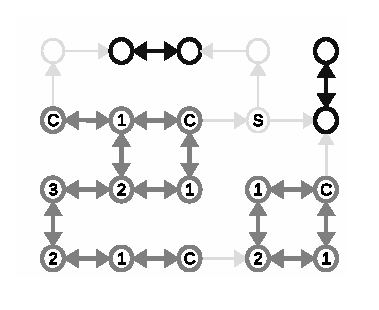
\includegraphics[scale=0.66]{fig/sd_graph_plateaus_ordered}}\\
  \subfloat[]{\protect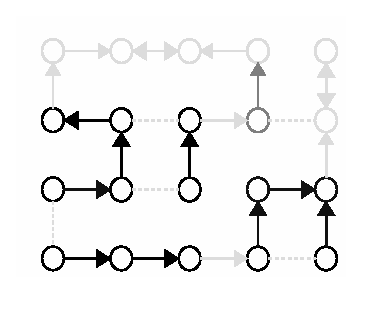
\includegraphics[scale=0.66]{fig/sd_graph_plateaus_modified}}
  \subfloat[]{\protect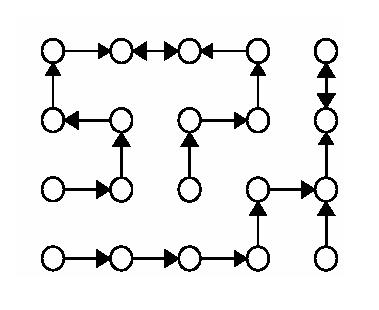
\includegraphics[scale=0.66]{fig/final_segmentation}}

  \protect\caption{(a) Vertex indices; (b) distances to the nearest
    plateau corner; (c) modifications to the steepest descent graph;
    (d) final watershed partition of the graph}
\end{figure}


\section{Watershed transform algorithm}

 We introduce an ordering function $\alpha:V\to\{1,2,...,|V|\}$ such
 that $\alpha(u)\neq\alpha(v)$ if and only if $u\neq v$. We'll refer
 to $\alpha(u)$ as the index of $u$ (Fig. 2(a)). In the first part of
 the algorithm we modify $D$ by removing edges. For all \emph{saddle
   vertices} we keep only one outgoing edge - the one pointing to a
 vertex with the lowest index. In the next step we divide the
 \emph{non-minimal plateaus}. We initialize a global FIFO queue $Q$,
 mark all the \emph{plateau corner} vertices as visited and insert
 them into $Q$ in increasing order of their index. While $Q$ is not
 empty we remove the vertex $v$ from the front of the queue, we then
 explore all the bidirectional edges $\{v,u\}$. If $u$ is not visited,
 we mark it as such, insert it to the back of the queue and change the
 edge to be incoming $(v\leftarrow u)$. Otherwise, if the vertex was
 already visited we just remove the edge. The resulting steepest
 descent graph is shown on Fig. 2(c) - the dotted edges are
 removed. Considering all the remaining edges as bidirectional, the
 connected components of the modified descent graph $D$ will be the
 \emph{watershed} \emph{basins of attraction}.

 The algorithm runs in linear time with respect to the number of edges
 in $G$ and produces an optimal partitioning as defined
 in~\cite{Cousty2009}. The total number of segments in the
 partitioning will equal to the total number of \emph{regional
   minima}. We defer the detailed algorithm listing, the proof of
 correctness and running time analysis to the supplementary material.


 We present the watershed transform algorithm from {\bf Section 2} of
 the main manuscript. We assume there is an ordering of the vertices
 in $V$. Usually the information about the vertices is stored in an
 array, where the $i$-th element of the array contains the vertex with
 index $i$.

\begin{enumerate}
\item Apply the threshold $T_{\min}$ and $T_{\max}$:
  \begin{enumerate}
  \item Remove each $\{u,v\}$ from $E$ if $w(\{v_i,u\}) > T_{\max}$.
  \item For each $\{u,v\}$ from $E$ set $w(\{v_i,u\}) = 0$ if
    $w(\{v_i,u\}) < T_{\min}$.
  \item Remove singleton vertices (vertices with no incident edges in
    $E$). Mark them as background.
  \end{enumerate}
\item Create $G'$. Set $V'=V$ and $E'=\emptyset$. For each vertex $v_i
  \in V'$:
  \begin{enumerate}
  \item Calculate $M_i = \min_{u \in V', \{v_i,u\} \in
    E}\{w(\{v_i,u\})\}$.
  \item For each $u \in V'$ such that $\{v_i,u\} \in E$ add $(v_i,u)$
    to $E'$ if $w(\{v_i,u\})=M_i$.
  \end{enumerate}
\item Modify $G'$ to remove all saddle vertices. For each vertex $v
  \in V$ that has more than one outgoing edge, keep only one outgoing
  edge pointing to a vertex with the minimal index.
\item Modify $G'$ to split the non-minimal plateaus:
  \begin{enumerate}
  \item Initialize a FIFO queue $Q$.
  \item For each vertex $v \in V'$, check whether the vertex has at
    least one outgoing edge and one bidirectional edge (check whether
    the vertex is a plateau corner). If it does mark it as visited and
    add it to the end of $Q$.
  \item While $Q \neq \emptyset$, let $u$ be the first element of $Q$
    and remove it from $Q$. For all $v$ such that $(u,v) \in E'$ and
    $(v,u) \in E'$ remove $(u,v)$ from $E'$. If $v$ is visited remove
    $(v,u)$ from $E'$ as well, otherwise mark $v$ as visited and add
    it to the end of $Q$.
  \end{enumerate}
\item Replace all unidirectional edges with bidirectional edges. For
  each $(u,v) \in E'$ add $(v,u)$ to $E'$ if not already there.
\item Return connected components of the modified $G'$.
\end{enumerate}

In the first step of the algorithm we apply the thresholds and mark
the singleton vertices as background, as desired by the output. We
expect all the other vertices to be assigned to a watershed basin. In
the second step we create the steepest descent graph. In the steps 3
we make sure that all the saddle vertices are removed. After this step
there will be no vertices with more than one outgoing edge. The step 4
splits the plateaus. In the breadth first search, while examining the
plateau vertices, we make sure that all the vertices have only one
outgoing edge. The breadth first search order will ensure that we keep
the edge on the path to the closest plateau corner (with the minimal
index). After the step 4 all vertices that don't belong to a regional
minima will have a single outgoing edge, hence there will be an unique
steepest descent path to a single regional minima. Therefore, all the
vertices will be uniquely assigned to a basin. The step 5 just makes
sure there's also a path from a regional minima to all vertices in its
basin of attraction so that we can just apply connected components in
order to obtain the watershed basins.

As we operate on a connected graph we assume $O(|E|) \ge O(|V|)$. The
first three steps of the algorithm visit each edge constant number of
times. In the step 4, we visit each vertex at most once. While
visiting each vertex we visit edges incident to it constant number of
times. The step 5 also visits each edge at most once. As the
complexity of connected components is $O(|E|)$, we get our overall
complexity to be $O(|E|)$.

\section{Reducing over-segmentation}.

 Noisy values of \emph{disaffinities} can produce severe
 over-segmentation (Fig. 3(c)). In order to reduce the
 over-segmentation we often merge adjacent segments with the
 \emph{saliency} below some given threshold
 $T_{\min}$~\cite{Najman1996}. The \emph{saliency} of two adjacent
 segments is defined as the value of the minimal \emph{disaffinity}
 between the vertices of the two segments. That means that we are
 confident that \emph{disaffinities} below $T_{\min}$ connect vertices
 of the same segment. An equivalent segmentation can be obtained by
 replacing the weights of all edges in $G$ with the weight smaller
 than $T_{\min}$ to a common low value (e.g. $0$) before applying the
 watershed transform. We prove this claim in the supplementary
 material. To show confidence about high values of
 \emph{disaffinities}, and in order to prevent undesired mergers, we
 introduce a threshold $T_{\max}$ by erasing all the edges from $G$
 with the weight higher than $T_{\max}$, and essentially setting them
 to $\infty$. The $T_{\max}$ threshold can produce singleton vertices
 in $G$. The singleton vertices are not assigned to any \emph{basin of
   attraction} and are considered background, which is often a desired
 result.

\begin{enumerate}
\item Applying watershed transform and then merging all basins with
  saliency smaller than $T_{\min}$, and
\item Applying watershed on a graph where with all the edges with
  weight smaller than $T_{\min}$ are replaced with edges with weight
  of $0$
\end{enumerate}
are equivalent. We first prove the following lemma:

\subsubsection{Lemma 1}
\emph{Examine a watershed transform $W$ of $G$ and watershed transform
  $W'$ obtained by applying a threshold $T_{\min}$ on $G$. Let
  $\{B_1,B_2,\dots\}$ be the watershed basins of $W$ and
  $\{B'_1,B'_2,\dots\}$ the watershed basins of $W'$. For each $B_i$
  there exist $B'_j$ such that $B_i \subseteq B'_j$}.


\subsubsection{Proof}.
The steepest descent graph containing only vertices in $V$ that are
not incident to any edge with the weight smaller than $T_{\min}$ will
stay unmodified, even after splitting the plateaus and getting rid of
the saddle vertices. All other vertices will became a part of a
regional minima (locally minimal plateau in the steepest descent
graph). All previous locally minimal edges will stay locally
minimal. Therefore applying the threshold $T_{\min}$ just introduces
bidirectional edges to the steepest descent graph. Therefore, a
connected component in the modified steepest descent graph of $G$ has
to be a subset of a connected component of the modified steepest
descent graph of $G$ after applying $T_{\min}$.

Watershed basins of $W'$ are connected. Hence, they can be obtained by
merging watershed basins of $W$. We prove that the result of 1. and
2. are equivalent by showing that two neighboring basins of $W$, $B_i$
and $B_j$ will be merged in 1. if and only if they are merged in 2.

Let's examine two watershed basins of $W$, $B_i$ and $B_j$. If there
is an edge $\{u,v\}$ in $G$ such that $u \in B_i$ and $v \in B_j$ with
the weight smaller than $T_{\min}$, then $u$ and $v$ will be part of
the same regional minima in $W'$. Hence, the two basins of $W$ belong
to a single basin of $W'$. We also know that the saliency between
$B_i$ and $B_j$ has to be smaller than $T_{\min}$, therefore they will
belong to the same segment when applying the algorithm 1. Similarly,
if the saliency $d_{ij}$ between $B_i$ and $B_j$ is below $T_{\min}$,
then there exist an edge $\{u,v\}$ in $G$ such that $u \in B_i$ and $v
\in B_j$ with the weight equal to $d_{ij} < T_{\min}$. Therefore $u$
and $v$ will be part of the same regional minima, and $B_i$ and $B_j$
will be part of the same watershed basin in $W'$.

%%%%%%%%%%%%%%%%%%%%%%%%%%%%%%%%%%%%%%%%%%%%%%%%%%%%%%%%%%%%%%%%%%%%%%%
%%%%%%%%%%%%%%%%%%%%%%%%%%%%%%%%%%%%%%%%%%%%%%%%%%%%%%%%%%%%%%%%%%%%%%%
%%
%% REFERENCES
%%
%%%%%%%%%%%%%%%%%%%%%%%%%%%%%%%%%%%%%%%%%%%%%%%%%%%%%%%%%%%%%%%%%%%%%%%
%%%%%%%%%%%%%%%%%%%%%%%%%%%%%%%%%%%%%%%%%%%%%%%%%%%%%%%%%%%%%%%%%%%%%%%


{\small
\bibliographystyle{ieeetr}
\bibliography{./ref/bib}
}

\end{document}
